\documentclass[12pt]{article}
\usepackage{graphicx}
\begin{document}

We processed the images using ANTs tools to segment deep gray matter,
CSF, white matter and cortical volume.   These measurements, for each
individual, were merged with demographics prepared by Laura
Betancourt. Jue Wu performed the image processing.  

We tested the full model with all covariates to determine whether
tissue volumes are related to the Adjusted HOME variable in the
presence of covariates accounting for gestational age, maternal age at
delivery and maternal BMI at delivery.  

\begin{table}[ht]
\centering
\begin{tabular}{rrrrr}
  \hline
 & Estimate & Std. Error & t value & Pr($>$$|$t$|$) \\ 
  \hline
(Intercept) & -38.4580 & 22.7634 & -1.69 & 0.1350 \\ 
  Cortex & -0.0006 & 0.0001 & -6.39 & 0.0004 \\ 
  deepGrayMatter & 0.0008 & 0.0006 & 1.24 & 0.2557 \\ 
  whiteMatter & 0.0007 & 0.0001 & 4.93 & 0.0017 \\ 
  csf & 0.0002 & 0.0000 & 4.39 & 0.0032 \\ 
  GestAge & 1.1885 & 0.6265 & 1.90 & 0.0996 \\ 
  BMIdel & -0.1710 & 0.0451 & -3.79 & 0.0068 \\ 
  MatAgeAtDel & 0.2617 & 0.1145 & 2.29 & 0.0562 \\ 
   \hline
\end{tabular}
\caption{Full ADJ\_HOMETotalScore regression model with primary
  covariates: Gestational Age, BMI at delivery and maternal age.  Head
  circumference covaries with the brain tissue measurements. \newline ADJ\_HOMETotalScore  $\approx$ Cortex $+$  deepGrayMatter  $+$  whiteMatter  $+$ csf  $+$
GestAge  $+$ BMIdel  $+$   MatAgeAtDel}
\end{table}

The results suggest that cortical volume is significantly related to
the HOME measurement.  Furthermore, HOME scores can be accuately
predicted by this collection of variables as shown in the
cross-validation study summarized in Figure~\ref{fig:fig1}.  This
suggests that the full model is not overfitting.  These results are
suprising given the small sample size.  One potential interpretation (if
results hold) is in line with our other HOME paper: variations within
low-SES homes directly impact brain development.  Normal variability within resource-starved environments may lead to
long-term consequences on outcome, potentially through early impact on
neural architecture.

\begin{figure}
    \centering  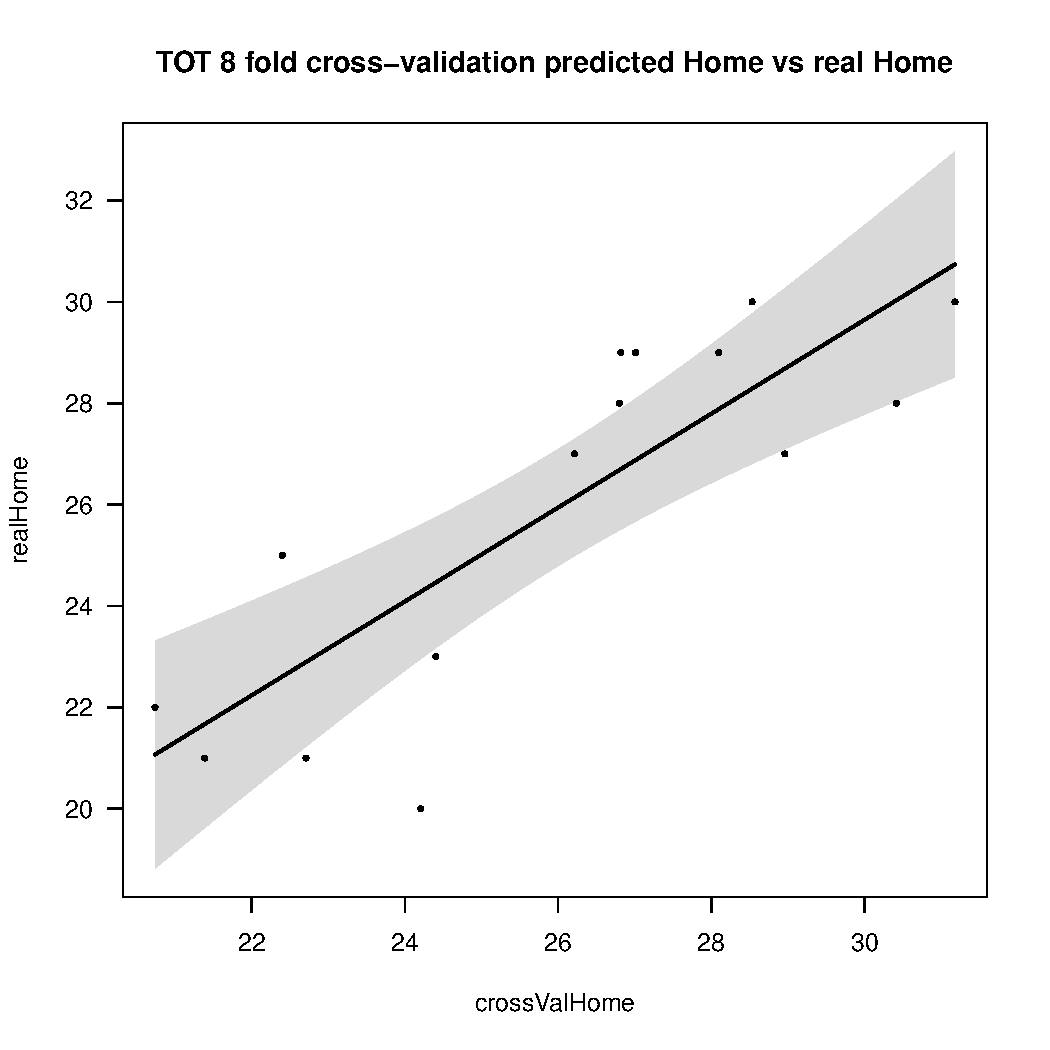
\includegraphics[width=5.5in]{TOT_8-fold_cross-validation_predicted_Home_vs_real Home.pdf}
    \caption{Predicted ADJ\_HOMETotalScore versus the real score using
      the 8-fold cross-validated version of the above full model.  1/8
    th of the data was held-out before predicting the remainder of the
  data.  This was repeated 8 times. \label{fig:fig1}}
    \label{simulationfigure}
\end{figure}

\end{document}
